\title{Solid State Physics: Final Exam Review}
\date{\today}

\documentclass[10pt]{article}
\usepackage{amsthm}
\usepackage{subcaption}
\usepackage{listings}
\usepackage{graphicx}
\usepackage{physics}

\graphicspath{ {figures/} }
\begin{document}
\maketitle

\section{LCAO and Tight Binding}
\subsection{Gentle Introduction: Covalent Bonding of Hydrogen Atoms}
Imagine a system in which two Hydrogen atoms are held with fixed-position nuclei
("Born-Oppenheimer Approximation") and a shared electron between them.
Goal: calculate the eigenenergies of the system as a funtion of the distance from the fixed nuclei.


The Hamiltonian of the system is given by

$$
H = K + V_{1} + V_{2}
$$

where
$$
K = \frac{\textbf{p}^{2}}{2m}
$$
and the coulombic potential due to the nucleus fixed at position $\textbf{R}_{i}$ is given by
$$
V_{i} = \frac{e^{2}}{4\pi\epsilon_{0}|\textbf{r} - \textbf{R}_{i}|}
$$
We can write down a trial solution of the form
$$
\ket{\psi} = \phi_{1}\ket{1} + \phi_{2}\ket{2}
$$
where $\ket{i}$ are the atomic orbitals (or ``tight-binding orbitals'') representing the
ground state solution for that particular isolated nucleus. That explicitly means the following
$$
(K + V_{1})\ket{1} = \epsilon_{0}\ket{1}
$$
$$
(K + V_{2})\ket{2} = \epsilon_{0}\ket{2}
$$
where $\epsilon_{0}$ is the ground state energy of a single Hydrogen atom.

In the LCAO/tight-binding method, we make the following approximation: \textbf{the
atomic orbitals $\ket{i}$ are orthogonal} such that
$$
\bra{i}\ket{j} = \delta_{ij}
$$
The Schrodinger equation can be written as
$$
H\ket{\psi} = E\ket{\psi}
$$
or, alternatively, in the $\ket{i}$ basis:
$$
\begin{bmatrix}
  H_{11} & H_{12} \\
  H_{21} & H_{22}
\end{bmatrix}
\begin{bmatrix}
  \phi_{1} \\
  \phi_{2}
\end{bmatrix}
 = E \begin{bmatrix}
   \phi_{1} \\
   \phi_{2}
 \end{bmatrix}
$$
By using a variational method where
$$
E = \frac{\bra{\psi}H\ket{\psi}}{\bra{\psi}\ket{\psi}}
$$
and
$$
\frac{\partial E}{\partial \phi_{i}} = \frac{\partial E}{\partial \phi_{i}*} = 0
$$
We obtain an eigenvalue equation
$$
\sum_{j}H_{ij}\phi_{j} = E\phi_{i}
$$
where $H_{ij} = \bra{i}H\ket{j}$. The components of $H$ can be written explicitly as
$$
H_{11} = \bra{1}H\ket{1} = \bra{1}K+V_{1}\ket{1} + \bra{1}V_{2}\ket{1} = \epsilon_{0} + V_{cross}
$$
$$
H_{22} = \bra{2}H\ket{2} = \bra{2}K+V_{2}\ket{2} + \bra{2}V_{1}\ket{2} = \epsilon_{0} + V_{cross}
$$$$
H_{12} = \bra{1}H\ket{2} = \bra{1}K+V_{2}\ket{2} + \bra{1}V_{1}\ket{2} = -t
$$$$
H_{21} = \bra{2}H\ket{1} = \bra{2}K+V_{1}\ket{1} + \bra{2}V_{2}\ket{1} = -t^*
$$
We make the following observations:
\begin{itemize}
  \item The on-site energy is given by
  $$\bra{i}K + V_{i}\ket{i} = \epsilon_{0}$$
  \item The coulombic potential due to site $j$ on site $i$ is given by
  $$\bra{i}V_{j}\ket{i} = V_{cross}$$
  \item The \emph{hopping term} is defined by
  $$\bra{j}V_{j}\ket{i} = \bra{i}V_{i}\ket{j}^* = -t$$
\end{itemize}

The eigenvalue equation then takes on the form of a $2\times 2$ matrix equation
$$
\begin{bmatrix}
  \epsilon_{0} + V_{cross} & -t \\
  -t^{*} & \epsilon_{0} + V_{cross}
\end{bmatrix}
\begin{bmatrix}
  \phi_{1} \\
  \phi_{2}
\end{bmatrix}
= E\begin{bmatrix} \phi_{1} \\ \phi_{2} \end{bmatrix}
$$
Diagonalization yields the eigenenergies
$$
E_{\pm} = \epsilon_{0} + V_{cross} \pm |t|$$

\subsection{Tight-Binding Chain}
In this section, we seek to observe that all waves in periodic environments behave similarly. Here
we consider electron waves, but we should consider the similarities to vibrational waves (phonons) as
well.

The one-dimensional tight binding has the following description.
\begin{itemize}
  \item There is a single orbital on atom $n$, denoted $\ket{n}$.
  \item Periodic boundary conditions are imposed such that $\ket{N} = \ket{0}$.
  \item Atomic orbital states are orthogonal.
  $$\bra{n}\ket{m} = \delta_{nm}$$
  \item The general trial wavefunction has the form
  $$\ket{\Psi} = \sum_{n}\phi_{n}\ket{n}$$
  \item The effective Schrodinger equation is
  $$
  \sum_{m}H_{nm}\phi_{m} = E\phi_{n}
  $$
  where $H_{nm} = \bra{n}H\ket{m}$.
  \item The Hamiltonian can be written
  $$
  H = K + \sum_{j}V_{j}
  $$
  where $K = \textbf{p}^{2}/2m$ and $V_{j} = V(\textbf{r} - \textbf{R}_{j})$.
\end{itemize}
Given the description above, we have
\begin{equation}
\begin{aligned}
  H\ket{m} & = (K + V_{m})\ket{m} + \sum_{j \neq m}V_{j}\ket{m} \\
           & = \epsilon_{atomic}\ket{m} + \sum_{j \neq m}V_{j}\ket{m}
\end{aligned}
\end{equation}
Therefore,
$$
H_{nm} = \bra{n}H\ket{m} = \epsilon_{atomic}\delta_{mn} + \sum_{j \neq m}\bra{n}V_{j}\ket{m}
$$
where
$$
\sum_{j \neq m}\bra{n}V_{j}\ket{m} = \left\{\begin{matrix}
 V_{0} & n=m \\
 -t & n=m\pm 1\\
 0 & 0
\end{matrix}\right.
$$
So,
$$
H_{n,m} = (\epsilon_{atomic} + V_{0})\delta_{nm} -t(\delta_{n+1,m} + \delta_{n-1,m}) = \epsilon_{0}\delta_{nm} -t(\delta_{n+1,m} + \delta_{n-1,m})
$$

\subsubsection{Solution}
We propose an ansatz
$$\phi_{n} = \frac{e^{-ikna}}{\sqrt{N}}$$
Note the absence of of a frequency component to the exponent, which is due
to the fact that we are seeking solutions to the time-independent Schrodinger
equation.
\begin{itemize}
  \item For a system with $N$ sites, and length $L = Na$, there are $N$ possible
  solutions of the ansatz form.
  \item Each solution corresponds to $k = 2\pi m/L$, where $m = 0, ..., N-1$.
\end{itemize}
Plugging the ansatz into the Schrodinger equation gives
\begin{equation}
\sum_{m}H_{nm}\phi_{m} = \epsilon_{0}\frac{e^{-ikna}}{\sqrt{N}} - t\left( \frac{e^{-ik(n+1)a}}{\sqrt{N}} + \frac{e^{-ik(n-1)a}}{\sqrt{N}}\right)
\end{equation}
and we also know that
\begin{equation}
  E\phi_{n} = E\frac{e^{-ikna}}{\sqrt{N}}
\end{equation}
Equating the previous two equations gives us
$$
E = \epsilon_{0} - 2t\cos(ka)
$$
(Note the correspondance to the phonon spectrum for the 1D monatomic chain). The dispersion curve is shown in Fig. 1.

\begin{figure}
  \centering
    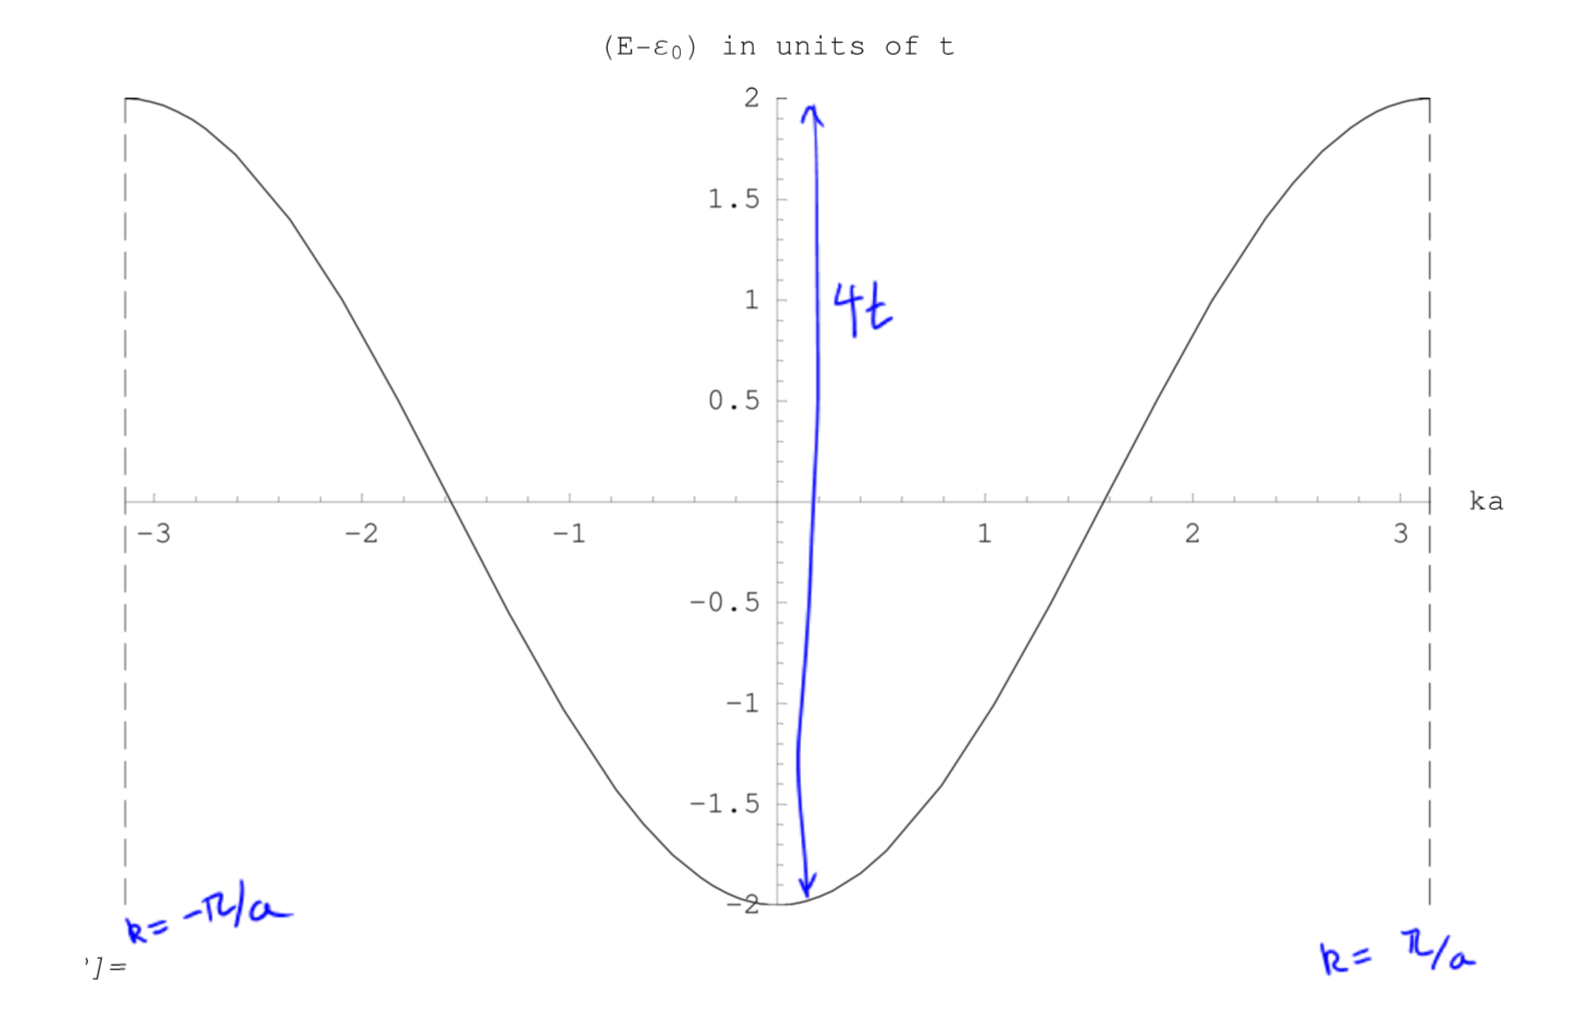
\includegraphics[width=\textwidth]{tb1}
    \caption{Dispersion curve for tight-binding chain.}
\end{figure}

Some notes about the dispersion relation:
\begin{itemize}
  \item The periodicity is $k \rightarrow k + \frac{2\pi}{a}$ (like phonons).
  \item Zero group velocity (flat curve) at the Brillouin zone boundary (like phonons).
  \item Electrons may only have eigenstates within a certain \emph{band}, referring to both
  the energy range in which the eigenstates exist as well as the individual branches
  of the dispersion curve itself.
  \item The \emph{bandwidth} refers to the difference between the maximum and minimum energies
  in a band. In Fig. 1, the bandwidth is $4t$.
  \item The bandwidth, $4t$, is dependent on the hopping amplitude and, therefore, on the
  interatomic spacing between nuclei. This dependence is shown in Fig. 2.
  \item As seen in Fig. 2, the effect of the hopping is to raise the energy of some eigenstates and lower the
  energy of others (such that the average is still $\epsilon_{0}$). If the band is not completely filled, then
  the average energy dips below $\epsilon_{0}$ since some higher states are not filled.
\end{itemize}

\begin{figure}
  \centering
    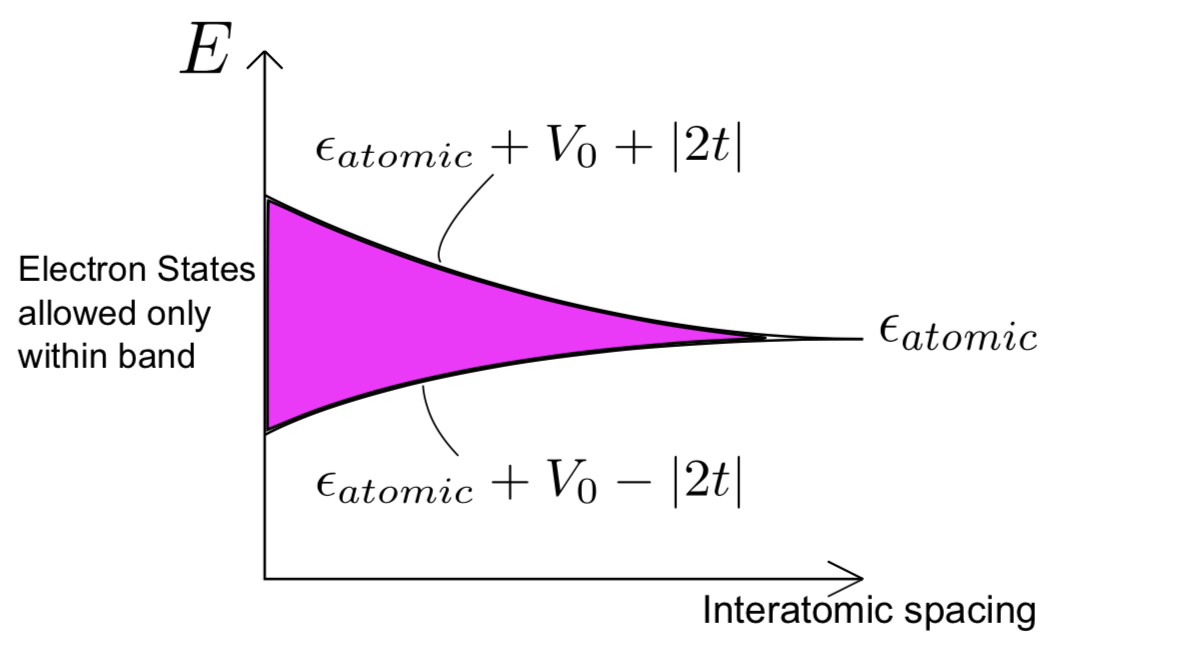
\includegraphics[width=\textwidth]{tb2}
    \caption{Bandwidth dependence on interatomic spacing.}
\end{figure}

Near the bottom of the band in Fig. 1, where $k$ is close to zero, the dispersion is approximately parabolic. For
small $k$, $cos(ka) \approx 1 - k^{2}a^{2}/2$, so

$$
E(k) \approx Constant + ta^{2}k^{2}
$$

\textbf{Note:} If the minimum were at the Brillouin zone edge, we would need to expand around $k = \pi/a$ instead.
Since the dispersion of the free electron can be written as
$$E_{free}(k) = \frac{\hbar^{2}k^{2}}{2m}$$
We can relate the two dispersion relations to calculate an \emph{effective mass} $m^{*}$ such that the dispersion at
the bottom of the band behaves as a free electron of mass $m^{*}$.
$$
\frac{\hbar^{2}k^{2}}{2m^{*}} = fa^{2}k^{2}
$$
and the effective mass is then
$$
m^{*} = \frac{\hbar^{2}}{2ta^{2}}
$$

\subsection{Band Filling}
\subsubsection{Monovalent Case}
If every atom in the one-dimensional, single-orbital tight binding model were to ``donate'' an electron,
then we would have a total of $N$ electrons. These electrons occupy the $N$ lowest-energy states in the band,
which has $N$ allowed eigenstates, but each eigenstate can be populated by a spin-up and a spin-down electron.
The band is therefore only half filled, as seen in the left of Fig. 3.

In Fig. 3, the Fermi surface (the energy level separating occupied and unoccupied states) is $\epsilon_{0}$. By providing a small bit of
energy, the Fermi sea can be shifted slightly such that the electrons take on an average net positive momentum (right side of Fig. 3) and
current is able to flow. For this reason, monovalent materials are frequently metals.

\begin{figure}
  \centering
    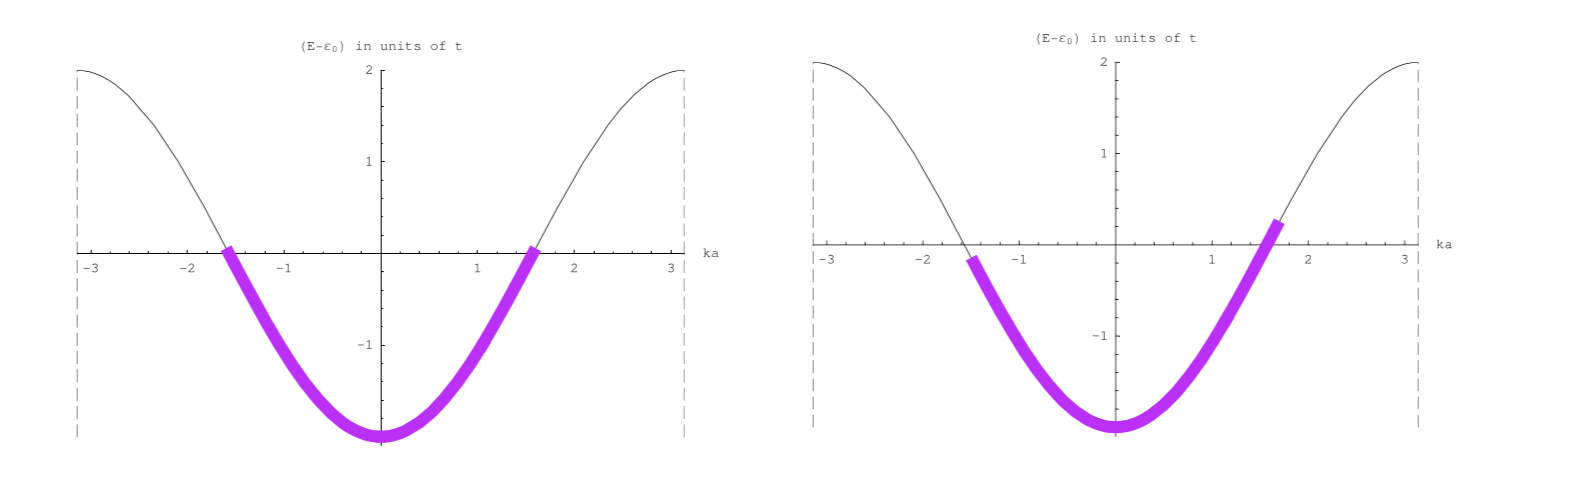
\includegraphics[width=\textwidth]{tb3}
    \caption{Monovalent Fermi surface and shifted Fermi sea.}
\end{figure}

\subsubsection{Divalent Case}
In the divalent case, there are a total of $2N$ atoms, which fill all spin-up and spin-down states of each of the $N$ allowed
eigenstates. That is, the band is completely filled. Therefore, there are no free $k$ states to which the Fermi sea could shift to allow a current to
be induced. \textbf{A filled band carries no current}. This results in a \emph{band insulator}.

\subsection{Multiple Bands}
In the one-dimensional, single-orbital tight-binding model, there is a single band. However, if we consider multiple
orbitals per unit cell, more bands will emerge. We may consider, for example:
\begin{itemize}
  \item Multi-atom unit cells with one or more orbitals each.
  \item Single-site unit cells with multiple orbitals per site.
\end{itemize}
The energy bandwidth as a function of inter-atomic spacing is shown in Fig. 4 for the case where there are two orbitals per single-site.
\begin{figure}
  \centering
    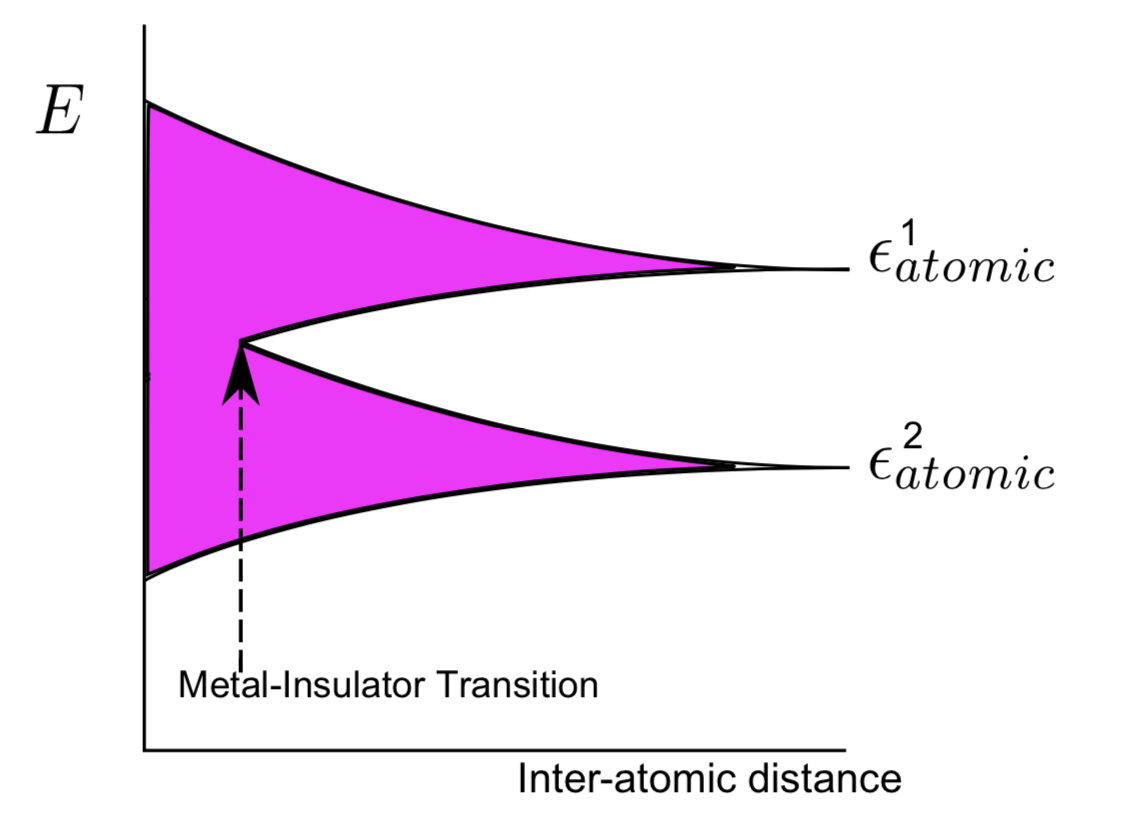
\includegraphics[width=\textwidth]{tb4}
    \caption{Energy bandwidth as a function of inter-atomic distance. Two atomic orbitals per site.}
\end{figure}
The dispersion relation for the two-site, single orbital case is shown in Fig. 5. Some notes:
\begin{itemize}
  \item If both species are divalent, then there are already a total of two electrons filled each orbital on every atom - that is,
  both branches of the dispersion are filled.
  \item If both species are monovalent, then only the bottom band is filled (i.e. only half the states are filled). So, there are $k$
  states available to shift the Fermi sea (around the Fermi surface, which is halfway between the top and bottom bands). However, to
  shift the sea, we need to apply an electric field strong enough to overcome the energy gap between the bands. \textbf{A filled band
  is an insulator as long as there is a finite gap to any higher-level band}.
  \item As seen in Fig. 4, as the interatomic distance decreases, the bandwidths of the individual bands come to overlap and there is no
  longer a gap between the lower- and higher-energy bands. In this limit, the material comes to behave as a metal.
\end{itemize}
\begin{figure}
  \centering
    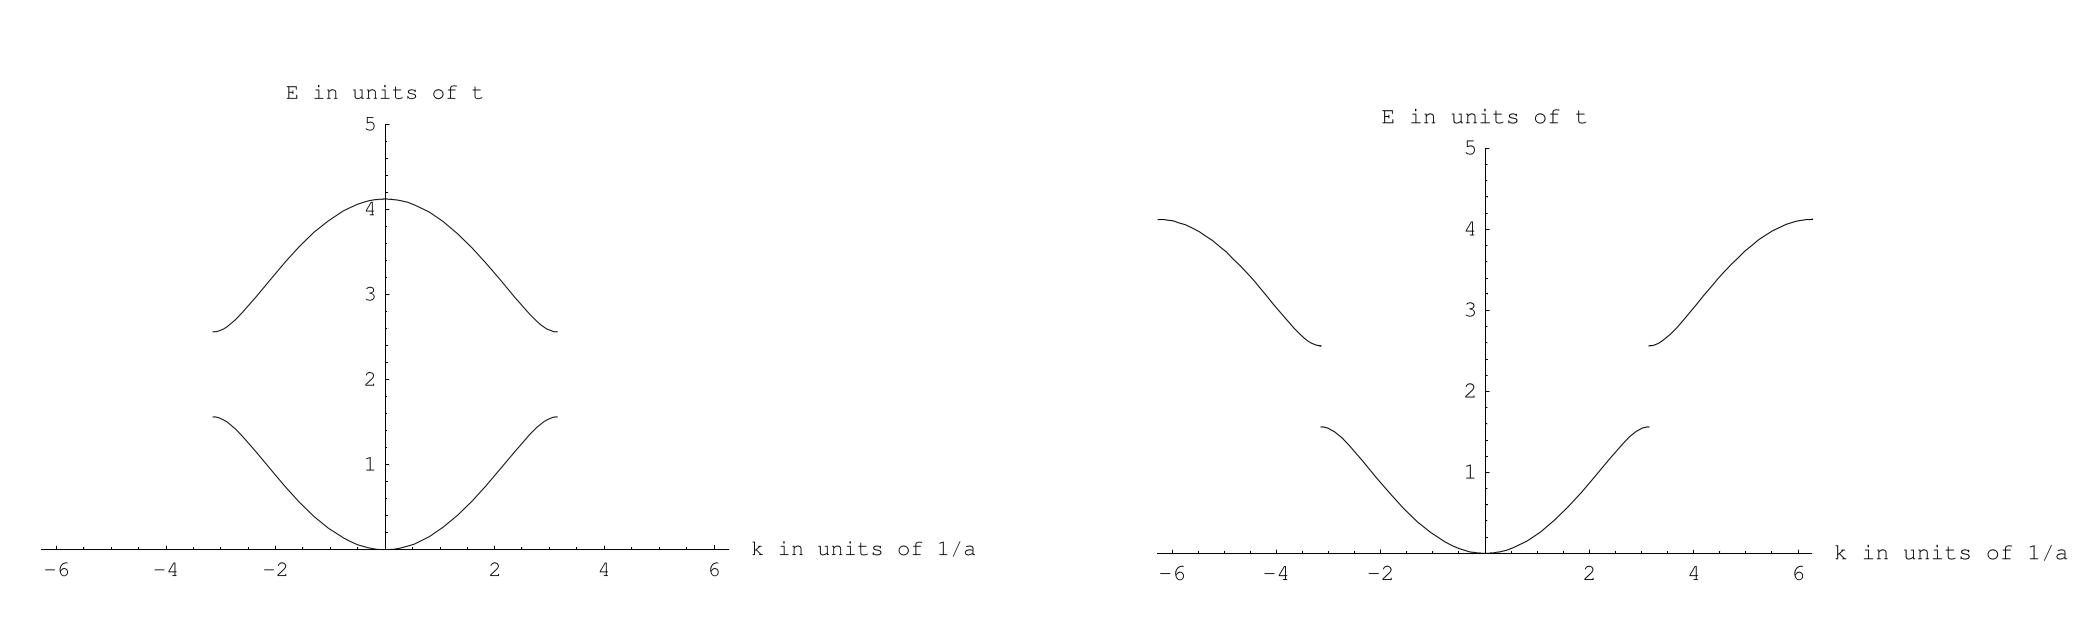
\includegraphics[width=\textwidth]{tb5}
    \caption{Dispersion relation for tight-binding model with two sites per unit cell, one orbital per site.}
\end{figure}

\section{Nearly Free Electron Model}

To do: Chapters 15, 16, 23, 17
\end{document}
